\documentclass[tikz,border=10pt]{standalone}
\usetikzlibrary{positioning,arrows.meta}

\begin{document}
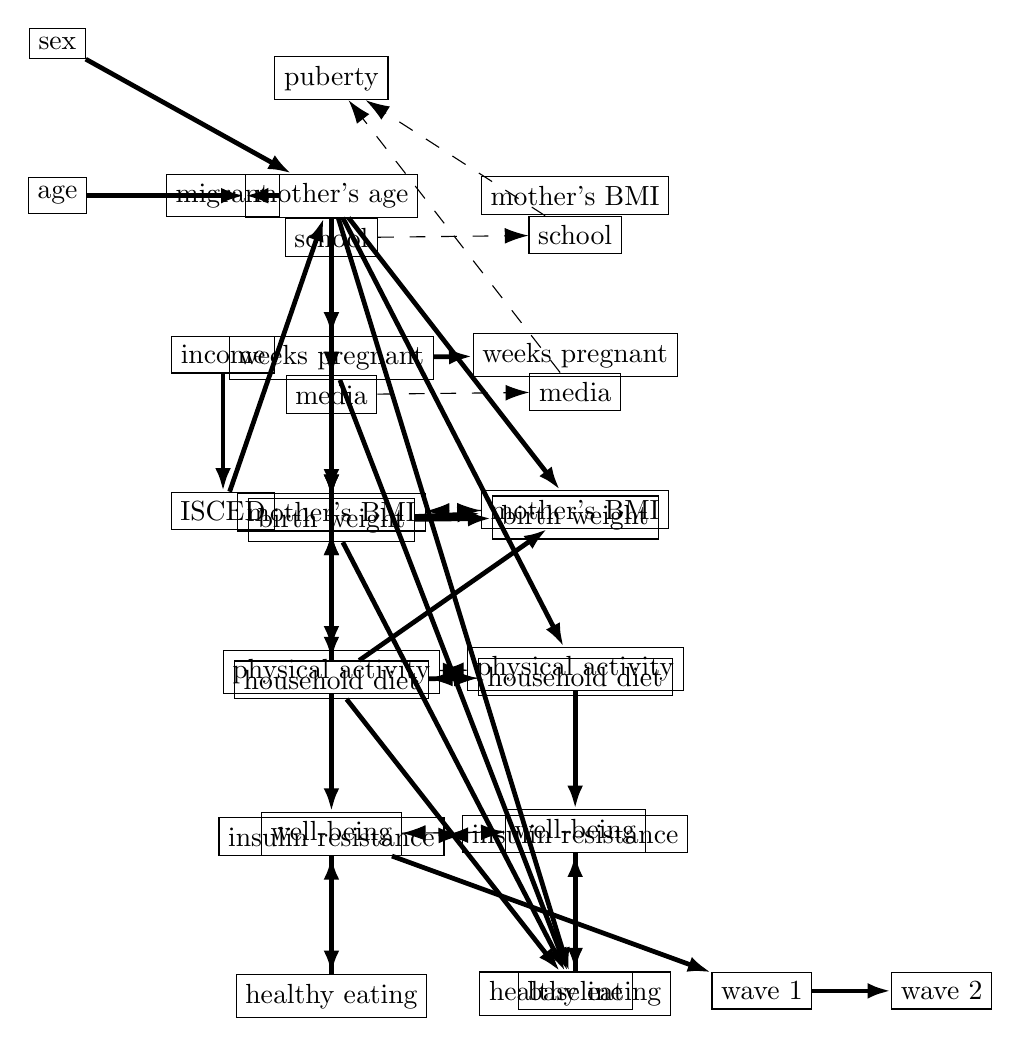
\begin{tikzpicture}[
    node distance=1.5cm and 1cm,
    every node/.style={draw, rectangle, align=center},
    bold edge/.style={line width=0.6mm, -{Latex[length=3mm, width=2mm]}},
    dotted edge/.style={dash pattern=on 2mm off 2mm, -{Latex[length=3mm, width=2mm]}},
]

% Nodes
\node (sex) {sex};
\node[below=of sex] (age) {age};
\node[right=of age] (migrant) {migrant};
\node[below=of migrant] (income) {income};
\node[below=of income] (ISCED) {ISCED};
\node[right=2cm of age] (motherage) {mother's age};
\node[below=of motherage] (weeks) {weeks pregnant};
\node[below=of weeks] (birthweight) {birth weight};
\node[below=of birthweight] (household) {household diet};
\node[below=of household] (insulin2) {insulin resistance};
\node[below=of insulin2] (healthy2) {healthy eating};
\node[above=of healthy2] (well2) {well-being};
\node[above=of well2] (physical2) {physical activity};
\node[above=of physical2] (BMI2) {mother's BMI};
\node[above=1cm of BMI2] (media) {media};
\node[above=of media] (school) {school};
\node[above=of school] (puberty) {puberty};

\node[right=5cm of age] (motherage2) {mother's BMI};
\node[below=of motherage2] (weeks2) {weeks pregnant};
\node[below=of weeks2] (birthweight2) {birth weight};
\node[below=of birthweight2] (household2) {household diet};
\node[below=of household2] (insulin1) {insulin resistance};
\node[below=of insulin1] (healthy1) {healthy eating};
\node[above=of healthy1] (well1) {well-being};
\node[above=of well1] (physical1) {physical activity};
\node[above=of physical1] (BMI1) {mother's BMI};
\node[above=1cm of BMI1] (media1) {media};
\node[above=of media1] (school1) {school};

\node[below=of well1] (baseline) {baseline};
\node[right=of baseline] (wave1) {wave 1};
\node[right=of wave1] (wave2) {wave 2};

% Edges
\draw[bold edge] (sex) -- (motherage);
\draw[bold edge] (age) -- (motherage);
\draw[bold edge] (migrant) -- (motherage);
\draw[bold edge] (income) -- (ISCED);
\draw[bold edge] (ISCED) -- (motherage);

\draw[bold edge] (motherage) -- (birthweight);
\draw[bold edge] (weeks) -- (birthweight);
\draw[bold edge] (birthweight) -- (BMI1);
\draw[bold edge] (birthweight) -- (BMI2);
\draw[bold edge] (household) -- (BMI1);
\draw[bold edge] (household) -- (BMI2);
\draw[bold edge] (weeks) -- (weeks2);
\draw[bold edge] (birthweight) -- (birthweight2);
\draw[bold edge] (household) -- (household2);
\draw[bold edge] (motherage) -- (weeks);
\draw[bold edge] (motherage) -- (birthweight);
\draw[bold edge] (motherage) -- (household);
\draw[bold edge] (motherage) -- (BMI1);
\draw[bold edge] (motherage) -- (BMI2);
\draw[bold edge] (motherage) -- (physical1);
\draw[bold edge] (motherage) -- (physical2);
\draw[bold edge] (physical1) -- (well1);
\draw[bold edge] (physical2) -- (well2);
\draw[bold edge] (well1) -- (healthy1);
\draw[bold edge] (well2) -- (healthy2);
\draw[bold edge] (healthy1) -- (insulin1);
\draw[bold edge] (healthy2) -- (insulin2);

\draw[dotted edge] (school) -- (school1);
\draw[dotted edge] (school1) -- (puberty);
\draw[dotted edge] (school) -- (media);
\draw[dotted edge] (media) -- (media1);
\draw[dotted edge] (media1) -- (puberty);
\draw[dotted edge] (BMI1) -- (BMI2);
\draw[dotted edge] (BMI2) -- (BMI1);
\draw[dotted edge] (well1) -- (well2);
\draw[dotted edge] (well2) -- (well1);
\draw[dotted edge] (physical1) -- (physical2);
\draw[dotted edge] (physical2) -- (physical1);
\draw[dotted edge] (household) -- (household2);
\draw[dotted edge] (household2) -- (household);
\draw[dotted edge] (insulin1) -- (insulin2);
\draw[dotted edge] (insulin2) -- (insulin1);

\draw[bold edge] (birthweight) -- (baseline);
\draw[bold edge] (weeks) -- (baseline);
\draw[bold edge] (motherage) -- (baseline);
\draw[bold edge] (household) -- (baseline);
\draw[bold edge] (well2) -- (wave1);
\draw[bold edge] (wave1) -- (wave2);

\end{tikzpicture}
\end{document}